\appendix

\section{Project directive and templates}
	
	\subsection{Contact information}
		\subsubsection{Customer}
			\begin{itemize}
				\item {\bf Nils Valland} \newline
						Telephone: 73 59 23 01 \newline
						Mobile: 92 41 20 37 \newline
						Fax: 73 59 22 40 \newline
						E-mail: nils.valland@artsdatabanken.no
				\item {\bf Askild Olsen} \newline
						Telephone: 73 59 21 93 \newline
						Mobile: 91 78 34 89 \newline
						Fax: 73 59 22 40 \newline
						E-mail: askild.olsen@artsdatabanken.no
			\end{itemize}
			
		\subsubsection{Supervisor}
			\begin{itemize}
				\item {\bf Muhammad Asif} \newline
						Telephone: 73 59 36 71 \newline
						E-mail: muhamma@idi.ntnu.no
			\end{itemize}

		\subsubsection{Team members}
				\begin{itemize}
					\item {\bf Anders Søbstad Rye} \newline
							E-mail: anderrye@stud.ntnu.no
					\item {\bf Andreas Berg Skomedal} \newline
							E-mail: andrskom@stud.ntnu.no
					\item {\bf Dag-Inge Aas} \newline
							E-mail: dagingaa@stud.ntnu.no
					\item {\bf Muhsin Gnaydin} \newline
							E-mail: gunaydin@stud.ntnu.no
					\item {\bf Nikola Djoric} \newline
							E-mail: nikoladj@stud.ntnu.no
					\item {\bf Stian Liknes} \newline
							E-mail: stianlik@stud.ntnu.no
					\item {\bf Yonathan Redda} \newline
							E-mail: redda@stud.ntnu.no
				\end{itemize}
	\newpage
	\subsection{Meeting agendas}
		\begin{figure}[htb]
			\centering
			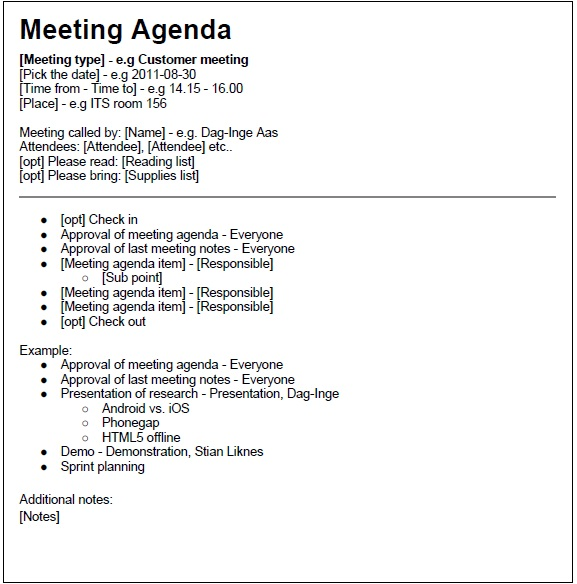
\includegraphics[width=0.8\textwidth]{appendix/meeting_agenda.jpg}
			\caption{Meeting agenda}
			\label{fig:meeting-agenda}
		\end{figure}
	
	\newpage
	\subsection{Meeting minutes}
		\begin{figure}[htb]
			\centering
			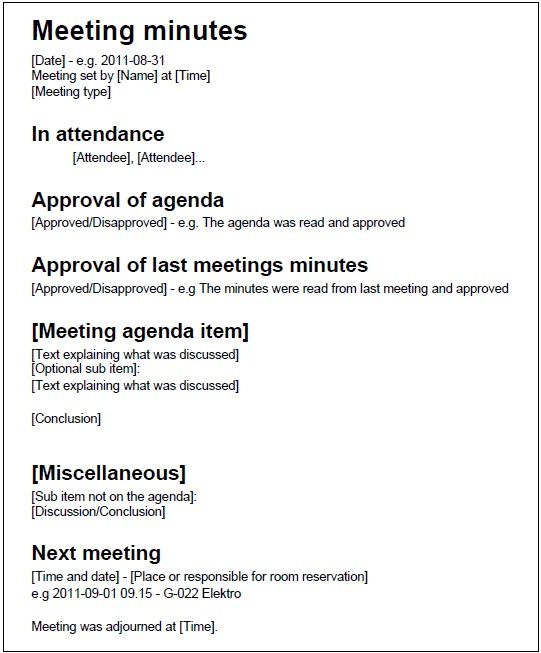
\includegraphics[width=0.8\textwidth]{appendix/meeting_minutes.jpg}
			\caption{Meeting minutes}
			\label{fig:meeting-minutes}
		\end{figure}
	
	\newpage
	\subsection{Weekly status report}
		\begin{figure}[htb]
			\centering
			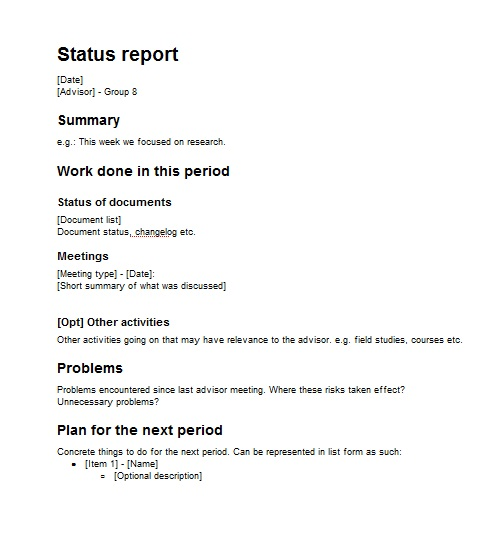
\includegraphics[width=0.8\textwidth]{appendix/weekly_status_report.jpg}
			\caption{Weekly status report}
			\label{fig:weekly-status-report}
		\end{figure}

\newpage
\section{User guide TODO}
This portion of the document details installation guides for the user, in addition to a how-to for the application. This should provide the user with adequate information about how to install and use the application.
\subsection{Installation guide}
The application can be downloaded from the Android Market, with the name "Artsdatabanken". It can also be installed directly from an executable installation package, an apk, by going to the following url: \url{http://stuff.daginge.com/artsdatabanken.apk}.

However, if the user wishes to install the latest build, see Developers guide.

\subsection{How-to}
\subsubsection{Creating an observation}
The user creates an observation by following the "Create and observation/Ny Observasjon" link from the front page of the application.
From here, the user selects which species group to observe. 
This will lead the user to an observation table, where the user can input species name, which is auto-completed, and the number of individuals found. 
Both common names and scientific names are applicable. 

\subsubsection{Add additional information}
From the observation page, the user can choose to add more information about the species observation by selecting "Add more information/Detaljer".

All fields are available for editing, simple to use boxes will open if date or time fields are edited.

\subsubsection{Add pictures of a species}
At the bottom of the Extended information page the user may also include images from disk or camera, if the user clicks on an already existing image he/she can remove the picture from the observation again.

\subsubsection{Adding additional species to an observation}
The user may also add additional species to an observation via the "Add additional species/Legg til ny art" button. This will create a new row for that species.

\subsubsection{Storing an observation}
To store an observation simply click the "Save/Lagre" button at the bottom of the observation.

\subsubsection{Editing a stored observation}
To edit an existing observation the user can select "Saved observations/Lagrede Observasjoner" from the front page. 
This will list all saved observations on the device. 
These observations are identifiable from it's species type, date of creation and an id assigned to it.

\subsubsection{Exporting an observation}
To export an observation the user can click on the "Export/Eksporter" button at the bottom of the observation page.
This will open up a menu to select which application to use for exporting, the recommended choice is an email client.
The user is free to send the observation to any email address, the received email can be used on the web-page of Artsdatabanken by copying the entire email body and pasting it in the import from XSL section.
Any images linked to the observation will be attached to the email.

\subsubsection{Deleting an observation}
An observation can be deleted by clicking the "Delete/Slett" button at bottom of an observation.

\section{Developers guide TODO}
This section will in details help maintaining developers understand and use the code we have produced during the course of this project. It will also include comments about the ideas we have for the further development of this app.

\subsection{Further work}
At this time this is a simple application for creating and submitting observations.
Improvements in design and functionality shouldn't be an issue, and the potential i present.
First priorities might be the incorporation of a direct submission API towards Artsdatabankens services, to avoid having to export through mail and import again.
Optimizing screen use might also be an idea, at the time objects are fairly large and space consuming, but this is more of a design philosophy from JQuery Mobile and is debatable.

Adding a section of the application for viewing species and obtain more information about them was a subject from the beginning of the project.
But it was of less importance and quickly deemed outside the scope of the original application.

At the current time most object methods are implemented functionally and not by using the "prototype" construct of JavaScript. 
At this point there isn't many concurrent objects in use at the same time so it shouldn't be much of an issue.
However as the application progresses this should most likely be changed to improve performance.

\subsubsection{Use of API}
Use of Artsdatabankens API in our application.
TODO STIAN

\subsubsection{Code repository}
The code and documentation from this project can be found in its entirety at the following url: \url{https://github.com/cdproject8/Artsdatabanken}. Included here is a complete revision history for our entire project, all of our documentation excluding meeting minutes and agendas, in addition to the app itself. The application is ready to compile from this source.

For further work, we recommend you fork this project. The project is licensed under Creative Commons Attribution-ShareAlike 3.0 Unported, and all further work should also be licensed under the same or similar licenses.

\subsubsection{Maintenance}
A short text about maintenance, and the challenges ahead.

\subsubsection{Not yet implemented and ideas}
Ideas for further development of the app from the project group and customer.
QUESTION isn't this the same as the further work section?

